\documentclass[paper=a4, fontsize=12pt]{scrartcl}
\usepackage[T1]{fontenc}
\usepackage{fourier}

\usepackage[english]{babel}															% English language/hyphenation
\usepackage[protrusion=true,expansion=true]{microtype}	
\usepackage{amsmath,amsfonts,amsthm} % Math packages
\usepackage[pdftex]{graphicx}	
\usepackage{url}


%%% Custom sectioning
\usepackage{sectsty}
\allsectionsfont{\centering \normalfont\scshape}


%%% Custom headers/footers (fancyhdr package)
\usepackage{fancyhdr}
\pagestyle{fancyplain}
\fancyhead{}											% No page header
\fancyfoot[L]{}											% Empty 
\fancyfoot[C]{}											% Empty
\fancyfoot[R]{\thepage}									% Pagenumbering
\renewcommand{\headrulewidth}{0pt}			% Remove header underlines
\renewcommand{\footrulewidth}{0pt}				% Remove footer underlines
\setlength{\headheight}{13.6pt}


%%% Equation and float numbering
\numberwithin{equation}{section}		% Equationnumbering: section.eq#
\numberwithin{figure}{section}			% Figurenumbering: section.fig#
\numberwithin{table}{section}				% Tablenumbering: section.tab#


%%% Maketitle metadata
\newcommand{\horrule}[1]{\rule{\linewidth}{#1}} 	% Horizontal rule

\title{
		%\vspace{-1in} 	
		\usefont{OT1}{bch}{b}{n}
		\normalfont \normalsize \textsc{CMSC 471 Artificial Intelligence UMBC} \\ [25pt]
		\horrule{0.5pt} \\[0.4cm]
		\huge Image Recognition in Machine Learning \\
		\horrule{2pt} \\[0.5cm]
}
\author{
		\normalfont 								\normalsize
        Brandon Walsh\\[-3pt]		\normalsize
        \today
}
\date{}


%%% Begin document
\begin{document}
\maketitle
\section{Problem}
Given a training set of images (dollar, hash, hat, heart, and smile) create a program that can take a filepath to a jpg and predict what the image is.

The goal is to maximize efficiency and accuracy by implementing the best suited machine learning algorithm.


\section{Approach}
There are three main parts to the image recognizer implemented in this project. This includes preprocessing images, simplifying the image data, and classifying the image data.

\subsection{Preprocessing Data}

All images first go through a preprocessor that converts them to 100x100 pixels and converts them to plain RGB values. This allows multiple image file types to be used. Each image is then converted to a numpy matrix. Each value in the matrix represents a 0-255 RGB value. This indicator will allow us to later classify the images. Let the matrix size be represented by nXm. The actual size of the matrix is 100x100x3 = 3000. This is because each pixel has 3 different values, red blue and green. In total there are 1000 pixels and 3000 data points. The matrix is then flattened into a numpy array, 1X(nxm). This allows for manipulation of the data using the scikit-learn toolkit.


\subsection{Simplify Image Data}
The goal is to use a classifier in order to group the training set of images. These predetermined classifications will be used in order to make future predictions. Supervised learning is the common terminology for this process. If the data is used as is after the preprocessor the classifier will have to work with 3000 dimensions per image. This is a large amount of data to store and process. It also does not allow for data visualization due to the high dimensionality.
We can significantly lower the dimensions while preserving the integrity of the data by using an algorithm known as Randomized Principle Component Analysis or Randomized PCA. Given a target number of dimensions the Randomized PCA algorithm will take the data from our flattened image array and simplify it to the target number of dimensions while preserving the integrity. This makes the data useful for the next step in the process, classification.


\subsection{Classify Data} 
Once the data is simplified and the number of dimensions has been lowered to something more reasonable, the data can be classified based on an associated label. This training process will allow non labeled images to be classified.
In this implementation a K-closest neighbors classifier is used. This algorithm simply finds K closest points based off of the training set and uses that information to determine the classification of the requested image.


\section{Program Accuracy}

The accuracy of the program is dependent on a few factors: the size of the training set, the number of features, and creator of the images. The most important factor is the size of the training set. The more images the program has to train from, the better the algorithm will be at making predictions. At the same time having too large of a training set could create some issues.  Each class could become too jagged and have difficulty distinguishing the classes. The program was tested with 30 images per class and 80 images per class. Classes with 30 images got 3/5 correct while classes with 80 images got 5/5 correct. A 2 dimensional graph of the class groupings is shown below along with a key. This data was simplified from 3000 to 2 features using the randomized PCA algorithm.

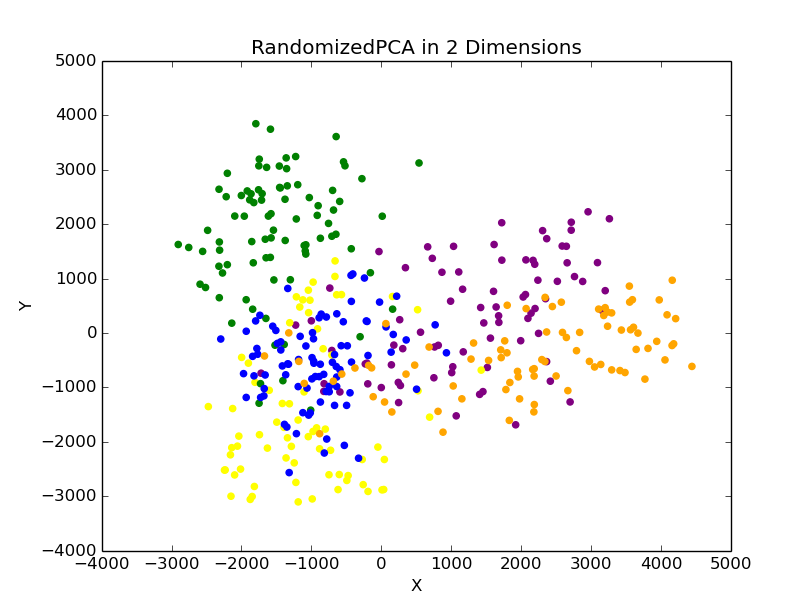
\includegraphics[width=\linewidth]{figure_1.png}
\paragraph{     Green=Dollar, Blue=Hash, Yellow=Hat, Purple=Heart, Orange=Smile\newline
\newline}

  
The number of features/dimensions played a large part in accuracy and how the data was classified. When the number of features was too high the k closest neighbours would commonly return the wrong value. When the number of features was too low, for example 2, the prediction was commonly wrong. 4 features seemed to be the most effective as it guessed the image correctly 100 percent of the time (based on my tests). The way the images are drawn have lots of variability. The 2 dimensional graph above shows how dollars and hashs have significant cross over. This can cause incorrect predictions on specific stylized images and make it more difficult for the program to choose the correct class.



%%% End document
\end{document}